
A table with subjects' answers was generated for each treatment. Table~\ref{table:example_table} is an example of the generated tables. 

\begin{table*}
\centering
\caption{Example of the table generated for each experience. This table corresponds to the experience with $ID=1$.}
\label{table:example_table}
\begin{tabular}{ | l | l | l | l | l | l | l | l | l | l | l | l |  }
\hline
	\rotatebox{90}{ \textbf{Sex}} & 
	\rotatebox{90}{ \textbf{Background}} & 
	\rotatebox{90}{ \textbf{Age}} & 
	\rotatebox{90}{ \textbf{Country of Origin}} & 
	\rotatebox{90}{ \textbf{Happy}} &
	\rotatebox{90}{ \textbf{Excited}} & 
	\rotatebox{90}{ \textbf{Tender}} & 
	\rotatebox{90}{ \textbf{Scared}} & 
	\rotatebox{90}{ \textbf{Angry}} & 
	\rotatebox{90}{ \textbf{Sad}} & 
	\rotatebox{90}{ \textbf{Other}} & 
	\rotatebox{90}{ \textbf{Explain}} \\ \hline
	Masculine & electronic engineering & 29 & Iran &  0 & 2 & 8 & 0 & 0 & 0 & 0 & \  \\ \hline
	Feminine & Computer science & 25 & Italy &  0 & 0 & 6 & 0 & 0 & 8 & 0 & \  \\ \hline
	Masculine & Computer science & 24 & Italy &  0 & 0 & 0 & 8 & 0 & 7 & 0 & \  \\ \hline
	Feminine & Pedagogical Science & 26 & Italy &  0 & 0 & 0 & 0 & 0 & 0 & 7 & Dubbioso \\ \hline
	Masculine & Computer science & 24 & Italy &  4 & 8 & 0 & 0 & 0 & 0 & 0 & \  \\ \hline
\multicolumn{12}{c}{}
\end{tabular}
\end{table*}

For each table were calculated mean, standard deviation, and median. It was not possible to use ANOVA test over the data because the assumption of normality is not satisfied in the collected data. This was checked using the Shapiro-Wilk Test.
Additionally, a contingency table for each emotion was generated in each treatment, as it is depicted in Table~\ref{table:table_contingency}, where the intensity for the rest of emotions is calculated as their mean of their intensity, including the option ``other''. Therefore a total of seven tables for each treatment were created. For all these tables, Krippendorff's alpha agreement~\cite{Krippendorff2007} ($\alpha$) was calculated, which is a reliability coefficient to measure the agreement among different participants. Unlike other coefficients (e.g., $Kappa$), $\alpha$ is a generalization of several known reliability indices, and it applies to any number of observers, any number of categories, any type of data, incomplete or missing data, large and small sample sizes.

This calculation was done using the R's package \textit{irr}. To improve contingency tables' interpretation, it was decided to just register emotions' alpha and intensity values greater than zero. The $\alpha$ for each treatment is shown in Figure~\ref{fig:alpha_experience}. As it could be observed, this table does not provide any information about the interpretation for each emotion. Therefore, it was decided to create top ten raking of treatments from the contingency tables of each emotion. This ranking is generated considering the following items in the respective order:(i) the mean intensity of the respective emotion, (ii) the alpha agreement of contingency table for the respective emotion, and (iii) the alpha agreement for the specific treatment. Table~\ref{table:happy_top_ten} for Happiness, Table~\ref{table:Angry_top_ten} for Anger, Table~\ref{table:Sad_top_ten} for Sadness, and Table~\ref{table:Scared_top_ten} for Fear.

\begin{figure*}
	\centering
	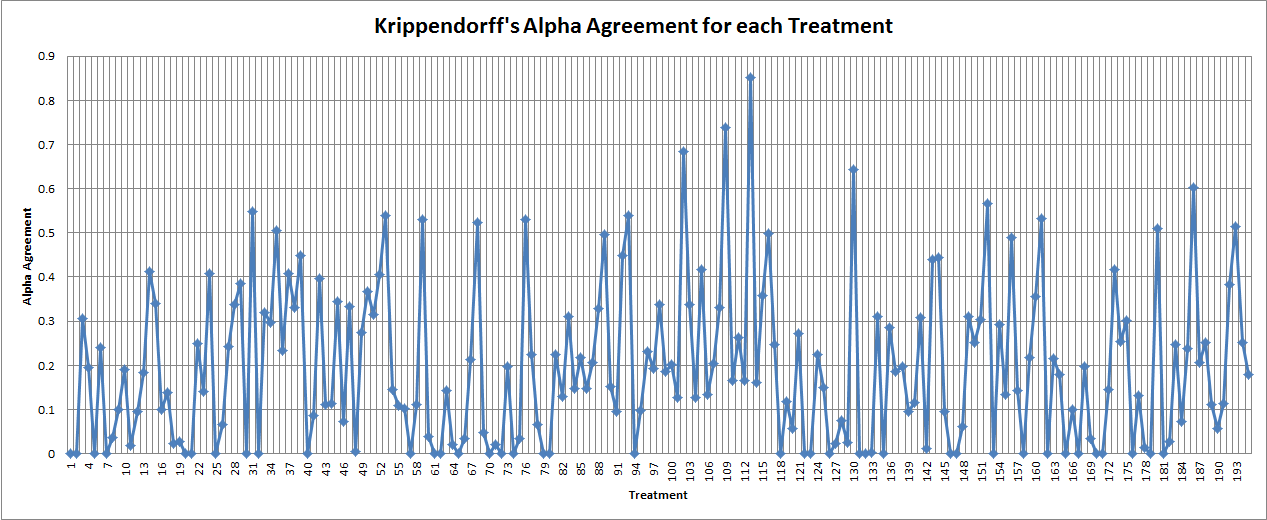
\includegraphics[width=1.0\textwidth]{./Images/Alpha.png} 
	\caption{Alpha values for each movement.}
	\label{fig:alpha_experience}
\end{figure*}

\begin{table}
\centering
\small
\caption{Top 10 attributions for Happiness.  This tops table was generated by ordering the results from highest to lowest first by Happy mean, then by Happy alpha, and finally by Movement alpha.}
\label{table:happy_top_ten}
\rotatebox{-90}{
\begin{tabular}{ | l | l | l | l | l | l | l | l | l | l | l | l | l | l | l | l | l | l | l | l |  }
\hline
\multicolumn{5}{|c|}{Features} & 
\multicolumn{8}{|c|}{Alpha} & 
\multicolumn{7}{c|}{Mean} \\ \hline
	\rotatebox{90}{\textbf{Direction (rad)}} &
	\rotatebox{90}{\textbf{Orientation (rad)}} & 
	\rotatebox{90}{\textbf{Linear V. (mm/sec)}} &
	\rotatebox{90}{\textbf{Angular V. (rad/sec)}} &
	\rotatebox{90}{\textbf{Angle (rad)}} &   
	\rotatebox{90}{\textbf{General}} & 
	\rotatebox{90}{\textbf{Happiness}} & 
	\rotatebox{90}{\textbf{Excitement}} & 
	\rotatebox{90}{\textbf{Tenderness}} & 
	\rotatebox{90}{\textbf{Fear}} & 
	\rotatebox{90}{\textbf{Anger}} & 
	\rotatebox{90}{\textbf{Sadness}} & 
	\rotatebox{90}{\textbf{Other}} & 
	\rotatebox{90}{\textbf{Happiness}} & 
	\rotatebox{90}{\textbf{Excitement}} & 
	\rotatebox{90}{\textbf{Tenderness}} & 
	\rotatebox{90}{\textbf{Fear}} & 
	\rotatebox{90}{\textbf{Anger}} & 
	\rotatebox{90}{\textbf{Sadness}} & 
	\rotatebox{90}{\textbf{Other}} \\ \hline
	0 & 0 & 500 & 3 & 0.349 &  0.38 & 0.71 & 0 & 0 & 0 & 0.13 & 0 & 0.13 & 6.8 & 3 & 2.6 & 0 & 1.4 & 0 & 1.4 \\ \hline
	$-\frac{\pi}{2}$ & 0 & 0 & 2 & 0.174 &  0.53 & 0.71 & 0 & 0 & 0 & 0 & 0 & 0 & 6.8 & 3.8 & 2 & 0 & 0 & 0 & 0 \\ \hline
	0 & 0 & 900 & 3 & 0.174 &  0.33 & 0.22 & 0 & 0.13 & 0 & 0 & 0 & 0 & 6.6 & 2.6 & 0.6 & 0 & 1.6 & 0 & 0 \\ \hline
	$\pi$ & $\pi$ & 0 & 3 & 0.349 &   0.21 & 0.21 & 0 & 0.13 & 0 & 0.23 & 0.34 & 0 & 6.6 & 3.6 & 1.4 & 2 & 0.8 & 0.4 & 0 \\ \hline
	$\pi$ & 0 & 900 & 3 & 0.349 &   0.48 & 0.11 & 0.72 & 0.12 & 0 & 0.76 & 0 & 0 & 6.4 & 6.8 & 1.2 & 4 & 0.2 & 0 & 0 \\ \hline
	0 & $\pi$ & 0 & 2 & 0.349 &  0.34 & 0.71 & 0 & 0 & 0.13 & 0.47 & 0.23 & 0 & 6 & 1.4 & 3.2 & 1.6 & 0.4 & 0.6 & 0 \\ \hline
	$\pi$ & $\pi$ & 0 & 2 & 0.174 &   0.31 & 0.12 & 0 & 0 & 0.61 & 0 & 0 & 0.13 & 6 & 4.8 & 4.8 & 0.4 & 0 & 0 & 2 \\ \hline
	$\pi$ & 0 & 500 & 2 & 0.349 &  0.43 & 0.11 & 0 & 0 & 0 & 0.13 & 0 & 0 & 6 & 0 & 3.4 & 0 & 0.6 & 0 & 2 \\ \hline
	0 & 0 & 500 & 1 & 0.174 &  0.24 & 0.11 & 0 & 0 & 0 & 0 & 0 & 0.13 & 6 & 4 & 4.2 & 0 & 2.2 & 0 & 1.2 \\ \hline
	$\pi$ & 0 & 200 & 3 & 0.349 &  0.28 & 0.22 & 0 & 0 & 0 & 0 & 0 & 0 & 5.8 & 0.8 & 3 & 0 & 0 & 0 & 1.4 \\ \hline
\multicolumn{16}{c}{}
\end{tabular}
}
\end{table}

\begin{table}
\centering
\small
\caption{Top 10 attributions for Anger. This tops table was generated by ordering from highest to lowest first by Angry mean, then by Angry alpha, and finally by Movement alpha.}
\label{table:Angry_top_ten}
\rotatebox{-90}{
\begin{tabular}{ | l | l | l | l | l | l | l | l | l | l | l | l | l | l | l | l | l | l | l | l |  }
\hline
\multicolumn{5}{|c|}{Features} & 
\multicolumn{8}{|c|}{Alpha} & 
\multicolumn{7}{c|}{Mean} \\ \hline
	\rotatebox{90}{\textbf{Direction (rad)}} &
	\rotatebox{90}{\textbf{Orientation (rad)}} & 
	\rotatebox{90}{\textbf{Linear V. (mm/sec)}} &
	\rotatebox{90}{\textbf{Angular V. (rad/sec)}} &
	\rotatebox{90}{\textbf{Angle (rad)}} &  
	\rotatebox{90}{\textbf{General}} & 
	\rotatebox{90}{\textbf{Happiness}} & 
	\rotatebox{90}{\textbf{Excitement}} & 
	\rotatebox{90}{\textbf{Tenderness}} & 
	\rotatebox{90}{\textbf{Fear}} & 
	\rotatebox{90}{\textbf{Anger}} & 
	\rotatebox{90}{\textbf{Sadness}} & 
	\rotatebox{90}{\textbf{Other}} & 
	\rotatebox{90}{\textbf{Happiness}} & 
	\rotatebox{90}{\textbf{Excitement}} & 
	\rotatebox{90}{\textbf{Tenderness}} & 
	\rotatebox{90}{\textbf{Fear}} & 
	\rotatebox{90}{\textbf{Anger}} & 
	\rotatebox{90}{\textbf{Sadness}} & 
	\rotatebox{90}{\textbf{Other}} \\ \hline
	0 & 0 & 0 & 2 & 0.087 & 0.19 & 0 & 0.13 & 0.13 & 0.13 & 0.22 & 0 & 0 & 3.2 & 1.4 & 1.2 & 1.8 & 6.4 & 0 & 0 \\ \hline
	0 & 0 & 900 & 2 & 0.087 & 0.29 & 0.13 & 0 & 0.76 & 0.13 & 0.21 & 0 & 0 & 1.6 & 3.8 & 0.2 & 1 & 6.4 & 0 & 0 \\ \hline
	$-\frac{\pi}{2}$ & 0 & 900 & 0 & 0 & 0.60 & 0 & 0 & 0 & 0.13 & 0.73 & 0 & 0 & 0 & 1.6 & 0 & 1.4 & 6.2 & 0 & 0 \\ \hline
	0 & 0 & 900 & 3 & 0.349 & 0.44 & 0 & 0 & 0 & 0 & 0.12 & 0 & 0 & 3 & 5 & 0 & 2.8 & 6.2 & 0 & 0 \\ \hline
	$-\frac{\pi}{2}$ & 0 & 200 & 3 & 0.087 & 0.41 & 0 & 0 & 0 & 0 & 0.11 & 0.47 & 0 & 0 & 4.8 & 2.6 & 0 & 5.8 & 0.4 & 0 \\ \hline
	$\pi$ & 0 & 500 & 3 & 0.087 & 0.44 & 0.13 & 0 & 0 & 0 & 0.43 & 0 & 0 & 0.8 & 2.6 & 0 & 1.4 & 5.2 & 0 & 0 \\ \hline
	0 & 0 & 200 & 3 & 0.087 & 0.13 & 0.13 & 0 & 0 & 0 & 0 & 0 & 0 & 1 & 0 & 0 & 2.4 & 5.2 & 0 & 1.8 \\ \hline
	0 & 0 & 900 & 1 & 0.087 & 0.54 & 0 & 0.16 & 0 & 0 & 0.16 & 0 & 0 & 2.4 & 6.4 & 0 & 0 & 5 & 0 & 0 \\ \hline
	0 & 0 & 900 & 0 & 0 & 0 & 0.13 & 0 & 0.13 & 0.13 & 0 & 0 & 0.13 & 1.6 & 3 & 1 & 1.6 & 5 & 0 & 1.8 \\ \hline
	$\pi$ & 0 & 500 & 2 & 0.087 & 0.30 & 0.13 & 0 & 0 & 0 & 0.21 & 0 & 0 & 1 & 1.8 & 0 & 3.4 & 4.8 & 0 & 0 \\ \hline
\multicolumn{16}{c}{}
\end{tabular}
}
\end{table}

\begin{table}
\centering
\small
\caption{Top 10 attributions for Fear.  This tops table was generated by ordering from highest to lowest first by Fear mean, then by Fear alpha, and finally by Movement alpha.}
\label{table:Scared_top_ten}
\rotatebox{-90}{
\begin{tabular}{ | l | l | l | l | l | l | l | l | l | l | l | l | l | l | l | l | l | l | l | l |  }
\hline
\multicolumn{5}{|c|}{Features} & 
\multicolumn{8}{|c|}{Alpha} & 
\multicolumn{7}{c|}{Mean} \\ \hline
	\rotatebox{90}{\textbf{Direction (rad)}} &
	\rotatebox{90}{\textbf{Orientation (rad)}} & 
	\rotatebox{90}{\textbf{Linear V. (mm/sec)}} &
	\rotatebox{90}{\textbf{Angular V. (rad/sec)}} &
	\rotatebox{90}{\textbf{Angle (rad)}} &
	\rotatebox{90}{\textbf{General}} & 
	\rotatebox{90}{\textbf{Happiness}} & 
	\rotatebox{90}{\textbf{Excitement}} & 
	\rotatebox{90}{\textbf{Tenderness}} & 
	\rotatebox{90}{\textbf{Fear}} & 
	\rotatebox{90}{\textbf{Anger}} & 
	\rotatebox{90}{\textbf{Sadness}} & 
	\rotatebox{90}{\textbf{Other}} & 
	\rotatebox{90}{\textbf{Happiness}} & 
	\rotatebox{90}{\textbf{Excitement}} & 
	\rotatebox{90}{\textbf{Tenderness}} & 
	\rotatebox{90}{\textbf{Fear}} & 
	\rotatebox{90}{\textbf{Anger}} & 
	\rotatebox{90}{\textbf{Sadness}} & 
	\rotatebox{90}{\textbf{Other}} \\ \hline
	$\pi$ & $\pi$ & 900 & 2 & 0.174 & 0.85 & 0 & 0 & 0.15 & 0.83 & 0 & 0 & 0 & 0 & 0 & 1.2 & 9.6 & 0 & 0 & 0 \\ \hline
	$\pi$ & $\pi$ & 900 & 1 & 0.087  & 0.73 & 0 & 0 & 0.15 & 0.79 & 0 & 0.79 & 0 & 0 & 0 & 0.6 & 9.6 & 0 & 0.2 & 0 \\ \hline
	$\pi$ & $\pi$ & 500 & 3 & 0.087 & 0.41 & 0.13 & 0 & 0 & 0.75 & 0 & 0 & 0 & 2 & 3.4 & 0 & 9 & 3.6 & 0 & 0 \\ \hline
	$\pi$ & $\pi$ & 500 & 2 & 0.174 & 0.33 & 0.24 & 0.24 & 0 & 0.34 & 0.24 & 0 & 0.25 & 1.33 & 1.5 & 0 & 7.83 & 0.66 & 0 & 1.66 \\ \hline
	$\pi$ & $\pi$ & 500 & 2 & 0.087 & 0.68 & 0 & 0 & 0 & 0.72 & 0.13 & 0 & 0 & 0 & 0 & 0 & 7.8 & 0.6 & 2.20 & 0 \\ \hline
	$\pi$ & $\pi$ & 200 & 2 & 0.087 & 0.44 & 0.13 & 0.13 & 0 & 0.66 & 0 & 0 & 0 & 1 & 1 & 1.2 & 7.6 & 1.6 & 0 & 0 \\ \hline
	$-\frac{\pi}{2}$ & 0 & 0 & 2 & 0.087 & 0.35 & 0.35 & 0.13 & 0 & 0.22 & 0 & 0 & 0 & 0.4 & 1.2 & 0 & 7.4 & 3 & 0 & 0 \\ \hline
	0 & $\pi$ & 900 & 3 & 0.087 & 0.53 & 0 & 0 & 0 & 0.30 & 0 & 0 & 0 & 0 & 0 & 0 & 7 & 2.20 & 0 & 0 \\ \hline
	$\pi$ & $\pi$ & 500 & 3 & 0.349 & 0.20 & 0.13 & 0.13 & 0 & 0.16 & 0.34 & 0 & 0 & 1.8 & 1.6 & 0 & 6.8 & 0.4 & 2.4 & 0 \\ \hline
	$\pi$ & $\pi$ & 200 & 2 & 0.174 & 0.53 & 0 & 0 & 0.13 & 0.71 & 0.13 & 0.13 & 0 & 0 & 0 & 1 & 6.6 & 0.8 & 1.2 & 0 \\ \hline
\multicolumn{16}{c}{}
\end{tabular}
}
\end{table}

\begin{table}
\centering
\small
\caption{Top 10 attributions for Sadness.  This tops table was generated by ordering from highest to lowest first by Sadness mean, then by Sadness alpha, and finally by Movement alpha.}
\label{table:Sad_top_ten}
\rotatebox{-90}{
\begin{tabular}{ | l | l | l | l | l | l | l | l | l | l | l | l | l | l | l | l | l | l | l | l |  }
\hline
\multicolumn{5}{|c|}{Features} & 
\multicolumn{8}{|c|}{Alpha} & 
\multicolumn{7}{c|}{Mean} \\ \hline
	\rotatebox{90}{\textbf{Direction (rad)}} &
	\rotatebox{90}{\textbf{Orientation (rad)}} & 
	\rotatebox{90}{\textbf{Linear V. (mm/sec)}} &
	\rotatebox{90}{\textbf{Angular V. (rad/sec)}} &
	\rotatebox{90}{\textbf{Angle (rad)}} &
	\rotatebox{90}{\textbf{General}} & 
	\rotatebox{90}{\textbf{Happiness}} & 
	\rotatebox{90}{\textbf{Excitement}} & 
	\rotatebox{90}{\textbf{Tenderness}} & 
	\rotatebox{90}{\textbf{Fear}} & 
	\rotatebox{90}{\textbf{Anger}} & 
	\rotatebox{90}{\textbf{Sadness}} & 
	\rotatebox{90}{\textbf{Other}} & 
	\rotatebox{90}{\textbf{Happiness}} & 
	\rotatebox{90}{\textbf{Excitement}} & 
	\rotatebox{90}{\textbf{Tenderness}} & 
	\rotatebox{90}{\textbf{Fear}} & 
	\rotatebox{90}{\textbf{Anger}} & 
	\rotatebox{90}{\textbf{Sadness}} & 
	\rotatebox{90}{\textbf{Other}} \\ \hline
	$\pi$ & 0 & 200 & 1 & 0.349 & 0.64 & 0 & 0 & 0 & 0 & 0.13 & 0.73 & 0.13 & 0 & 0 & 0 & 0 & 1.2 & 7.4 & 1.6 \\ \hline
	0 & $\pi$ & 0 & 1 & 0.349 & 0.39 & 0 & 0 & 0.13 & 0 & 0 & 0.22 & 0 & 0 & 0 & 1.8 & 0 & 0 & 7.2 & 3.2 \\ \hline
	0 & 0 & 200 & 1 & 0.349 & 0.18 & 0.13 & 0 & 0 & 0 & 0.13 & 0.11 & 0 & 1.6 & 2 & 5.4 & 2.6 & 1.6 & 6 & 0 \\ \hline
	$-\frac{\pi}{2}$ & 0 & 200 & 0 & 0 & 0.10 & 0.13 & 0.29 & 0 & 0 & 0 & 0 & 0 & 0.8 & 0.4 & 1.8 & 0 & 0 & 6 & 3.2 \\ \hline
	$\pi$ & $\pi$ & 200 & 1 & 0.349 & 0 & 0 & 0 & 0.13 & 0.13 & 0.14 & 0 & 0 & 0 & 0 & 0.6 & 1.4 & 1.2 & 6 & 2.4 \\ \hline
	0 & $\pi$ & 200 & 0 & 0 & 0.27 & 0.13 & 0 & 0 & 0 & 0 & 0.21 & 0 & 1.2 & 0 & 3.4 & 1.8 & 0 & 5.8 & 0 \\ \hline
	$-\frac{\pi}{2}$ & 0 & 0 & 1 & 0.087 & 0.14 & 0 & 0.13 & 0.13 & 0.13 & 0 & 0.21 & 0.13 & 0 & 2 & 2 & 1.2 & 0 & 5.8 & 1.6 \\ \hline
	0 & $\pi$ & 200 & 1 & 0.349 & 0.40 & 0 & 0.13 & 0 & 0 & 0 & 0.57 & 0.13 & 0 & 0.8 & 3 & 3 & 0 & 5.6 & 0.6 \\ \hline
	$\pi$ & $\pi$ & 200 & 0 & 0 & 0.32 & 0.69 & 0.69 & 0 & 0 & 0 & 0.16 & 0 & 0.2 & 0.2 & 1.2 & 3.2 & 0 & 5.4 & 0 \\ \hline
	0 & $\pi$ & 200 & 1 & 0.087 & 0.36 & 0 & 0 & 0 & 0 & 0 & 0.16 & 0 & 0 & 0 & 3.6 & 3.6 & 0 & 5.4 & 0 \\ \hline
\multicolumn{16}{c}{}
\end{tabular}
}
\end{table}


\begin{table}
\caption{Contingency table formula used for each emotion and experience. Where $k$ is the kth experience, $j$ is jth emotion for the kth experience, $n$ is the total number of participants, and $Value$ is the intensity given by a participant.}
\label{table:table_contingency}
\small
\begin{tabular}{|l|l|l|}
\hline
Participant & Desire Emotion & Other Emotions \\
\hline
$1$ & $Value_{k,j}^{1}$  & $\frac{\sum_{i=1}^{i<=7 \wedge i \neq j}(Value_{k,i}^{1})}{\sum_{i=1}^{i<=6 \wedge i \neq j}(1)}$\\
\hline
$2$ & $Value_{k,j}^{2}$ & $\frac{\sum_{i=1}^{i<=7 \wedge i \neq j}(Value_{k,i}^{2})}{\sum_{i=1}^{i<=6 \wedge i \neq j}(1)}$\\
\hline
... & ... & ...\\
\hline
$n$ & $Value_{k,j}^{n}$ & $\frac{\sum_{i=1}^{i<=7 \wedge i \neq j}(Value_{k,i}^{2})}{\sum_{i=1}^{i<=6 \wedge i \neq j}(1)}$\\
\hline
\multicolumn{3}{c}{}
\end{tabular}
\end{table}